\chapter[Lagrangian Mechanics]{Lagrange and Euler-Lagrange mechanics}
In this section we will discuss the main possible formulations of classical mechanics and their derivations. We also want to note that all the formulations are derived from Newton's equations and so they are completely equivalent to them if the conditions for their validity are satisfied.
\section{Lagrange equations}
Going back to \dalembertref, expressing in generalized coordinates:
\begin{equation}
    \bigsum_i \brackets{\vec{F}^{\cancel{(a)}}_i - \dvec{p}_i} \cdot \delta \vec{r}_i = 0
\end{equation}
We drop the (a) term for an easier notation, from now on we will write $\vec{F}_i$ knowing that we are indicating the applied force.
\begin{equation}
    \delta \vec{r}_i = \bigsum_{\alpha} \pdv{ \vec{r}_i}{ q_{\alpha}} \delta q_{\alpha} + \cancel{\pdv{ \vec{r}_i}{ t} \dd{t}}
\end{equation}
The partial derivative over time is zero since we are considering a fixed moment in time. The force term in \dalembertref\;becomes:
\begin{equation}
    \bigsum_i \vec{F}_i \cdot \bigsum_{\alpha} \pdv{ \vec{r}_i}{ q_{\alpha}} \delta q_{\alpha} = \bigsum_{\alpha}\underbrace{\bigsum_{i} \vec{F}_i \cdot \pdv{ \vec{r}_i}{ q_{\alpha}}}_{Q_{\alpha}} \delta q_{\alpha} = \bigsum_{\alpha}Q_{\alpha}\delta q_{\alpha}
\end{equation}
The terms $Q_{\alpha}$ are called \textbf{generalized components of the forces}.
Now let's consider the expression $\bigsum_i \dvec{p}_i \cdot \delta \vec{r}_i$. We know that:
\begin{itemize}
    \item $\dvec{p}_i = \dv{}{t}\brackets{m_i\vec{v}_i}$
    \item $\delta \vec{r}_i = \bigsum_{\alpha} \pdv{ \vec{r}_i}{ q_{\alpha}}\delta q_{\alpha}$
\end{itemize}
Now, from the product rule:
\begin{equation} \label{e:total_deriv}
    \dv{}{t}\brackets{m_i\vec{v}_i \cdot \pdv{ \vec{r}_i}{ q_{\alpha}}} = \dv{}{t}\brackets{m_i\vec{v}_i}\cdot \pdv{ \vec{r}_i}{ q_{\alpha}} + m_i\vec{v}_i \cdot \dv{}{t}\brackets{\pdv{ \vec{r}_i}{ q_{\alpha}}}
\end{equation}
From the last term we get:
\begin{equation} \label{e:funny_derivative_p1}
    \begin{split}
      m_i\vec{v}_i \cdot \dv{}{t}\brackets{\pdv{ \vec{r}_i}{ q_{\alpha}}} &= m_i\vec{v}_i \cdot \bigsum_{\beta} \pdv{}{ \dot{q}_{\beta} }\brackets{\pdv{ \vec{r}_i}{ q_{\alpha}}} q_{\beta} + \pdv{}{ t}\brackets{\pdv{ \vec{r}_i}{ q_{\alpha}}} = \\[8pt]
      &= m_i\vec{v}_i \cdot \pdv{}{ q_{\alpha} }\underbrace{\sqbr{\bigsum_{\beta} \pdv{ \vec{r}_i}{ q_{\beta}} \dot{q}_{\beta} + \pdv{ \vec{r}_i}{ t}}}_{\vec{v}_i} = m_i\vec{v}_i \cdot \pdv{ \vec{v}_i}{ q_{\alpha}}
    \end{split}
\end{equation}
We now aim to prove that the partial derivative with respect to alpha in the first term in \eqref{e:total_deriv} is:
\begin{equation}
    \pdv{ \vec{r}_i}{ q_{\alpha}} = \pdv{ \vec{v}_i}{ \dot{q}_{\alpha}}
\end{equation}
Deriving what we got in \eqref{e:funny_derivative_p1} we get:
\begin{equation}
    \begin{split}
      \pdv{ \vec{v}_i}{ \dot{q}_{\alpha}} &= \pdv{ }{ \dot{q}_{\alpha}} \brackets{\bigsum_{\beta}\pdv{ \vec{r}_i}{ q_{\beta}} \dot{q}_{\beta} + \pdv{ \vec{r}_i}{ t}} = \\[8pt]
      &= \bigsum_{\beta}\pdv{ \vec{r}_i}{ q_{\beta}} \underbrace{\pdv{ \dot{q}_{\beta}}{ \dot{q}_{\alpha}}}_{\delta_{\alpha \beta}}  + \cancel{\pdv{ }{ \dot{q}_{\alpha}}\brackets{\pdv{ \vec{r}_i}{ t}}} = \pdv{ \vec{r}_i}{ q_{\alpha}}
    \end{split}
\end{equation}
Again, the first term of \eqref{e:total_deriv} can be rewritten as:
\begin{equation}
    \bigsum_i \dv{}{t}\brackets{m_i\vec{v}_i \cdot \pdv{ \vec{r}_i}{ q_{\alpha}}} = \bigsum_i\dv{}{t}\brackets{m_i\vec{v}_i \cdot \pdv{ \vec{v}_i}{ \dot{q}_{\alpha}}} = \dv{}{t}\sqbr{\pdv{ }{ \dot{q}_{\alpha}} \underbrace{\bigsum_i \brackets{\dfrac{1}{2}m_i \vec{v}_i \cdot \vec{v}_i}}_{T}}
\end{equation}
Similarly the last term in \eqref{e:total_deriv} is:
\begin{equation}
    \bigsum_im_i\vec{v}_i \cdot \pdv{ \vec{v}_i}{ q_{\alpha}} = \pdv{ }{ \dot{q}_{\alpha}} \underbrace{\bigsum_i \brackets{\dfrac{1}{2}m_i \vec{v}_i \cdot \vec{v}_i}}_{T}
\end{equation}
So we get:
\begin{equation}
    \bigsum_i \dv{}{t}\brackets{m_i\vec{v}_i}\cdot \pdv{ \vec{r}_i}{ q_{\alpha}} = \dv{}{t}\pdv{ T}{ \dot{q}_{\alpha}} - \pdv{ T}{ q_{\alpha}}
\end{equation}
Going back to \dalembertref\;we get:
\begin{equation}
    \begin{split}
      \bigsum_i \brackets{\vec{F}_i - \dvec{p}_i} \cdot \delta \vec{r}_i &= \bigsum_{\alpha}Q_{\alpha}\delta q_{\alpha} - \bigsum_i \dv{}{t}\brackets{m_i\vec{v}_i} \cdot \bigsum_{\alpha}\pdv{ \vec{r}_i}{ q_{\alpha}}\delta q_{\alpha} = \\[8pt]
      &= \bigsum_{\alpha}Q_{\alpha}\delta q_{\alpha} - \bigsum_{\alpha}\bigsum_i \dv{}{t}\brackets{m_i\vec{v}_i} \cdot \pdv{ \vec{r}_i}{ q_{\alpha}}\delta q_{\alpha} = \\[8pt]
      &= \bigsum_{\alpha}Q_{\alpha}\delta q_{\alpha} - \bigsum_{\alpha}\brackets{\dv{}{t}\pdv{ T}{ \dot{q}_{\alpha}} - \pdv{ T}{ q_{\alpha}}}\delta q_{\alpha} = 0
    \end{split}
\end{equation}
All the terms are independent by construction so we get a set of equations which are called \textbf{Lagrange equations} $\heartsuit$:
\begin{equation} \label{Lagrange_equations}
    \boxed{\dv{}{t}\pdv{ T}{ \dot{q}_{\alpha}} - \pdv{ T}{ q_{\alpha}} = Q_{\alpha}}
\end{equation}
which must be satisfied $\forall \alpha$s.
Here are some basic properties of \lagrangeref :
\begin{itemize}
    \item There is a minimum of $n$ equations to solve
    \item They are $2^\circ$ order differential equations, this means that for every equation we need 2 initial conditions
    \item There is a total of $2n$ total initial conditions
\end{itemize}
\section{Euler-Lagrange equations}
From \lagrangeref\;it is easy to derive another formulation. Suppose that every force is expressed through a potential:
\begin{equation}
    \vec{F}_i = -\nabla_i V
\end{equation}
Since $V$ (the total potential) must be a function of only the coordinates $V = V(\vec{r}_i)$ we get that:
\begin{equation}
    Q_{\alpha} = \bigsum_i \vec{F}_i \cdot \pdv{ \vec{r}_i}{ q_{\alpha}} = - \bigsum_i \nabla_i V \cdot \pdv{ \vec{r}_i}{ q_{\alpha}} = -\pdv{V}{q_{\alpha}}
\end{equation}
Rewriting \lagrangeref\;we get:
\begin{equation}
    \dv{}{t}\pdv{ T}{ \dot{q}_{\alpha}} - \pdv{ T}{ q_{\alpha}} + \pdv{V}{q_{\alpha}} = 0
\end{equation}
If the potential does not depend on the generalized velocities we can subtract its derivative with respect to $\dot{q}_{\alpha}$, which will just be 0:
\begin{equation}
    \dv{}{t}\pdv{ }{ \dot{q}_{\alpha}}[\underbrace{T-V}_\lagr ] - \pdv{}{ q_{\alpha}}[\underbrace{T-V}_\lagr ] = 0
\end{equation}
We define the Lagrange function or \textbf{Lagrangian} as:
\begin{equation}
    \lagr  = T - V
\end{equation}
Finally we can write the \textbf{Euler-Lagrange equations}:
\begin{equation} \label{Euler_Lagrange_equations}
    \boxed{\dv{}{t}\pdv{\lagr}{\dot{q}_{\alpha}} = \pdv{\lagr}{q_{\alpha}}}
\end{equation}
Here are some basic properties of \eleref :
\begin{itemize}
    \item They are $2^\circ$ order differential equations
    \item There is a total of $2n$ total initial conditions
    \item $\lagr = \lagr(q_{\alpha},\dot{q}_{\alpha},t)$ which means we have $2n+1$ variables
    \item $[\lagr] = \mathrm{J}$ but the Lagrangian is not the mechanical energy, it is just a mathematical tool
    \item If $\lagr$ is a Lagrangian of the system then $\tilde{\lagr} = \lagr + \mathrm{constant}$ is still a Lagrangian
    \item If $\lagr$ is a Lagrangian of the system and $F\in \mathcal{C}^1$ is an arbitrary function of \underline{coordinates and time} then $\tilde{\lagr} = \lagr + \partial_t F$ is a Lagrangian
\end{itemize}
If we have two system, let's call them $A$ and $B$ then the Lagrangian of the total system $AB$ in general \underline{is not}:
\begin{equation}
    \lagr_{AB} = T_A + T_B - V_A - V_B - \underbrace{V_{AB}}_{\text{interaction term}}\neq \lagr_A + \lagr_B
\end{equation}
but if the systems interact weakly then:
\begin{equation}
    \lagr_{AB} \approx \lagr_A + \lagr_B
\end{equation}
If the potential $V$ \underline{does not} depend on time explicitly then the system is conservative:
\begin{equation}
    \begin{split}
      \delta W &= \bigsum_i \vec{F}_i \delta \vec{r}_i = \bigsum_i \vec{F}_i \bigsum_{\alpha}\pdv{ \vec{r}_i}{ q_{\alpha}}\delta q_{\alpha} = \bigsum_{\alpha} Q_{\alpha}\delta q_{\alpha} = \\[8pt]
      &= -\bigsum_{\alpha} \pdv{V}{q_{\alpha}}\delta q_{\alpha} = -\dd{V}
    \end{split}
\end{equation}
Instead if $V$ \underline{depends} on time explicitly we have that:
\begin{equation}
    \dd{V} = \bigsum_{\alpha} \pdv{V}{q_{\alpha}}\delta q_{\alpha} + \pdv{ V}{ t}\dd{t}
\end{equation}
The extra term appearing in $\dd{V}$ is not present in the expression for work, meaning that:
\begin{equation}
    W_{12} \neq -\int_{1}^{2}\dd{V} = V_1 - V_2
\end{equation}
so the system is not conservative.\\
In some cases (ex. Lorentz force) the force does not come from a "real" potential, we can then rewrite \eleref\;for a function called \textbf{generalized potential} $\mu$ such that:
\begin{equation}
    Q_{\alpha} = -\pdv{ \mu}{ q_{\alpha}} +\dv{}{t}\pdv{ \mu}{ \dot{q}_{\alpha}}
\end{equation}
Indeed, from \lagrangeref\;we get:
\begin{equation}
    \begin{split}
      \dv{}{t}\pdv{ T}{ \dot{q}_{\alpha}} - \pdv{ T}{ q_{\alpha}} &= -\pdv{ \mu}{ q_{\alpha}} +\dv{}{t}\pdv{ \mu}{ \dot{q}_{\alpha}} \\[8pt]
      \dv{}{t}\pdv{ }{ \dot{q}_{\alpha}}[\underbrace{T-\mu}_{\lagr}] &- \pdv{}{ q_{\alpha}}[\underbrace{T-\mu}_{\lagr}] = 0 \\[8pt]
      \dv{}{t}\pdv{\lagr}{\dot{q}_{\alpha}} &= \pdv{\lagr}{q_{\alpha}}
    \end{split}
\end{equation}
where we defined a generalized Lagrangian $\lagr = T-\mu$. These are called \textbf{generalized Euler-Lagrange equations}.
\section{Derivation of Euler-Lagrange equations from Hamilton's principle}
A \textbf{monogenic system} is any system in which all the forces can be expressed through a (generalized) potential which depends on $q_{\alpha}$, $\dot{q}_{\alpha}$ and $t$.
\begin{definition}{Configuration space}
  Configuration space is the set of all the $q_{\alpha}$. It completely describes the position of each particle of the system at a givent time which, indeed, is the configuration of the system itself.
\end{definition}
We can imagine the configuration space as an $n$-dimensional space in which the axes are the various $q_{\alpha}$.
Since each $q_{\alpha}$ changes with respect to time, the system describes a curve in the configuration space.\\
Let us consider two instants of time $t_1$ and $t_2$:
\begin{figure}[H]
    \centering
    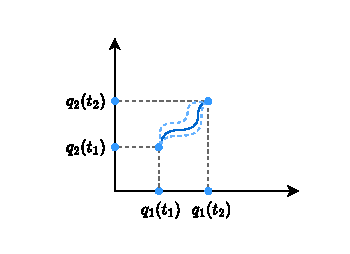
\includegraphics[width=0.6\linewidth]{res/svg/leastactionpath.drawio}
    \caption{Path of least action}
    \label{fig:image9}
\end{figure}
Then \textbf{Hamilton's principle} states that:
\begin{quote} \label{q:Hamilton_principle_quote} %Need to add principle ambient
    The path followed by a monogenic system in configuration space between $t_1$ and $t_2$ is the one for which the action $\action$ is stationary
\end{quote}
The action is defined as:
\begin{equation}
    \action = \int_{t_1}^{t_2}\lagr(q_{\alpha},\dot{q}_{\alpha},t) \dd{t}
\end{equation}
The units for actions are $[\action] = \mathrm{J\cdot s}$.\\ $\action$ is a \underline{functional} which is a "number" that depends on $q_{\alpha}$. Saying that $\action$ is stationary means that slightly changing the path does not change the action.\\
Now we aim to prove that the \hyperref[q:Hamilton_principle_quote]{Hamilton's principle} is true if and only if the \eleref\;are true.\\
\underline{Proof} H.P. $\Rightarrow$ E.L.E.\\
Let's give some conditions:
\begin{itemize}
    \item Call $\Gamma$ the real path
    \item Fix $t_1$ and $t_2$ but sligthly change the path in between
\end{itemize}
For the second point we need to change the real path of a small virtual displacement:
\begin{equation}
    q_{\alpha}(t) \longrightarrow q_{\alpha}(t) + \delta q_{\alpha}(t)
\end{equation}
However after varying the whole path, for the real path we get:
\begin{equation}
    \dot{q}_{\alpha} = \dfrac{\dd{q_{\alpha}}}{\dd{t}}
\end{equation}
for the changed path instead:
\begin{equation}
    \begin{split}
      \dot{q}_{\alpha} + \delta \dot{q}_{\alpha}(t) &= \dv{}{t}\brackets{q_{\alpha}(t) + \delta q_{\alpha}(t)} \\[8pt]
      \cancel{\dot{q}_{\alpha}} + \delta \dot{q}_{\alpha}(t) &= \cancel{\dot{q}_{\alpha}} + \dv{}{t}\brackets{\delta q_{\alpha}(t)} \\[8pt]
      \delta \dot{q}_{\alpha}(t) &= \dv{}{t}\brackets{\delta q_{\alpha}(t)}
    \end{split}
\end{equation}
Now let's evaluate the change on $\action$ and apply \hpquoteref\;which can be mathematically expressed as follows.\\\textbf{Hamilton's principle}:
\begin{equation} \label{e:Hamilton_principle}
    \delta \action = 0
\end{equation}
For the real path:
\begin{equation}
    \action = \int_{t_1}^{t_2}\lagr(q_{\alpha},\dot{q}_{\alpha},t) \dd{t}
\end{equation}
For the changed path:
\begin{equation}
    \tilde{\action} = \int_{t_1}^{t_2}\lagr(q_{\alpha}+\delta q_{\alpha},\dot{q}_{\alpha} + \delta \dot{q}_{\alpha},t) \dd{t}
\end{equation}
And so we get:
\begin{equation}
    \delta \action = \tilde{\action} - \action = \int_{t_1}^{t_2}\brackets{\lagr(q_{\alpha}+\delta q_{\alpha},\dot{q}_{\alpha} + \delta \dot{q}_{\alpha},t) - \lagr(q_{\alpha},\dot{q}_{\alpha},t)} \dd{t}
\end{equation}
The right-hand side of the equation basically has the numerator of the difference quotient:
\begin{equation}
    f'(x)h \sim f(x+h) - f(x)
\end{equation}
for arbitrarily small values of h, which in our case is the value of the virtual displacement $\delta$. Hence, we get:
\begin{equation}
    \delta \action = \int_{t_1}^{t_2}\bigsum_{\alpha}\brackets{\pdv{\lagr}{q_{\alpha}}\delta q_{\alpha} + \pdv{\lagr}{\dot{q}_{\alpha}} \underbrace{\delta \dot{q}_{\alpha}}_{\frac{\dd{}}{\dd{t}}\delta q_{\alpha}}} \dd{t} = 0
\end{equation}
Let's evaluate the second using integration by parts:
\begin{equation}
    \int_{t_1}^{t_2}\bigsum_{\alpha}\pdv{\lagr}{\dot{q}_{\alpha}} \dv{}{t}\delta q_{\alpha} \dd{t} = \cancel{\bigsum_{\alpha}\pdv{\lagr}{\dot{q}_{\alpha}} \delta q_{\alpha}\bigg|_{t_1}^{t_2}} - \int_{t_1}^{t_2}\bigsum_{\alpha}\dv{}{t}\brackets{\pdv{\lagr}{\dot{q}_{\alpha}}} \delta q_{\alpha} \dd{t}
\end{equation}
The term cancelled is zero since the displacement is zero in $t_1$ and $t_2$ for hypotesis. Hence, we get:
\begin{equation}
    \int_{t_1}^{t_2}\bigsum_{\alpha}\pdv{\lagr}{q_{\alpha}}\delta q_{\alpha} \dd{t} - \int_{t_1}^{t_2}\bigsum_{\alpha}\dv{}{t}\brackets{\pdv{\lagr}{\dot{q}_{\alpha}}} \delta q_{\alpha} \dd{t} = 0
\end{equation}
Since all the $\delta q_{\alpha}$ are independent we can pick any index $k$ and say that all the virtual displacements are zero except for the $k$-displacement, and we get:
\begin{equation}
    \int_{t_1}^{t_2}\pdv{ \lagr}{ q_{k}}\delta q_{k} \dd{t} - \int_{t_1}^{t_2}\dv{}{t}\brackets{\pdv{ \lagr}{ \dot{q}_{k}}} \delta q_{k} \dd{t} = 0
\end{equation}
Now we need a result which is called \textbf{Fundamental Lemma of the calculus of variation} which states that:\\
Taking any continuous function $M\in\mathcal{C}^0([a,b])$ and any function $\eta \in \mathcal{C}^2([a,b])$ such that $\eta(a) = \eta(b) = 0$ then it is true that:
\begin{equation} \label{e:Fundamental_lemma_variation_calculus}
    \int_{a}^{b}M(x)\eta(x)\dd{x} = 0 \Rightarrow M(x) = 0
\end{equation}
In our case \eqref{e:Fundamental_lemma_variation_calculus} is satisfied for:
\begin{equation}
    \int_{t_1}^{t_2}\underbrace{\sqbr{\pdv{ \lagr}{ q_{k}} - \dv{}{t}\brackets{\pdv{ \lagr}{ \dot{q}_{k}}}}}_{M} \underbrace{\delta q_{k}}_{\eta} \dd{t} = 0
\end{equation}
Hence:
\begin{equation}
    \begin{split}
      &\pdv{\lagr}{q_{\alpha}} - \dv{}{t}\brackets{\pdv{\lagr}{\dot{q}_{\alpha}}} = 0 \\[8pt]
      &\pdv{\lagr}{q_{\alpha}} = \dv{}{t}\brackets{\pdv{\lagr}{\dot{q}_{\alpha}}}
    \end{split}
\end{equation}
For any arbitrary $\alpha$. Hence, we proved that \hpquotemath\;implies \eleref.\\
It's trivial to prove the opposite since, repeating the passages of the first proof we arrive to:
\begin{equation}
    \delta \action = \int_{t_1}^{t_2}\bigsum_{\alpha}\sqbr{\pdv{\lagr}{q_{\alpha}} - \dv{}{t}\brackets{\pdv{\lagr}{\dot{q}_{\alpha}}}} \delta q_{\alpha}
\end{equation}
But the terms in the brackets are all zero because of the \eleref. So we get:
\begin{equation}
    \delta \action = 0
\end{equation}
Which is precisely \hpquotemath.\\
Now that we established the relations between the \eleref\;and the \hpquotemath\;we are ready to prove that if $\lagr$ is a Lagrangian:
\begin{equation}
    \tilde{\lagr} = \lagr + \dv{F}{t}
\end{equation}
is a Lagrangian for the system. Evaluating the action for both Lagrangians we get:
\begin{equation}
    \tilde{\action} = \int_{t_1}^{t_2}\lagr \dd{t} + \int_{t_1}^{t_2}\dfrac{\dd{F}}{\dd{t}} \dd{t}
\end{equation}
\begin{equation}
    \action = \int_{t_1}^{t_2}\lagr \dd{t}
\end{equation}
The difference of action for the new Lagrangian is:
\begin{equation}
    \delta \tilde{\action} = \int_{t_1}^{t_2}\dfrac{\dd{F}}{\dd{t}} \dd{t} = F(t_2) - F(t_1)
\end{equation}
And so we get:
\begin{equation}
    \delta \tilde{\action} = \delta \action + \cancel{\delta(F(t_2) - F(t_1))}
\end{equation}
The variation between the values of $F$ is obviously zero since their difference is just a constant number that comes from the integral. So if \hpquotemath\;holds for $\lagr$ we have:
\begin{equation}
    \delta \tilde{\action} = \delta \action = 0
\end{equation}
And so $\tilde{\lagr}$ is a Lagrangian for the system.\\
\section{Examples (WIP)}
\section{The energy function}
Let's now discuss the energy of a system. The Lagrangian $\lagr$ has the dimensions of an energy, but it \underline{is not} the total energy.
\begin{equation}
    \lagr = T - V \quad \cancel{\Leftrightarrow} \quad E = T + V
\end{equation}
We can evaluate the derivative of the Lagrangian and see what we get:
\begin{equation}
    \dfrac{\dd{\lagr}}{\dd{t}} = \bigsum_{\alpha}\brackets{\pdv{\lagr}{q_{\alpha}}\dot{q}_{\alpha} + \pdv{\lagr}{\dot{q}_{\alpha}}\ddot{q}_{\alpha}} + \pdv{ \lagr}{ t}
\end{equation}
If \eleref\;hold then we have:
\begin{equation}
    \dfrac{\dd{\lagr}}{\dd{t}} = \bigsum_{\alpha}\underbrace{\sqbr{\dv{}{t}\brackets{\pdv{\lagr}{\dot{q}_{\alpha}}}\dot{q}_{\alpha} + \pdv{\lagr}{\dot{q}_{\alpha}}\ddot{q}_{\alpha}}}_{\text{total time derivative}} + \pdv{ \lagr}{ t} =
\end{equation}
\begin{equation}
 = \dv{}{t}\bigsum_{\alpha}\pdv{\lagr}{\dot{q}_{\alpha}}\dot{q}_{\alpha} + \pdv{ \lagr}{ t}
\end{equation}
So in general:
\begin{equation}
    \dfrac{\dd{\lagr}}{\dd{t}} \neq 0
\end{equation}
even if the partial derivative of $\lagr$ with respect to time is zero. But we can define a quantity $h$ called \textbf{energy function}:
\begin{equation}
    h \defineeq \bigsum_{\alpha}\pdv{\lagr}{\dot{q}_{\alpha}}\dot{q}_{\alpha} - \lagr
\end{equation}
and so we have:
\begin{equation}
    \dfrac{\dd{h}}{\dd{t}} = -\pdv{ \lagr}{ t}
\end{equation}
Obviously $h$ is a constant of motion if and only if the partial derivative with respect to time of the Lagrangian is 0:
\begin{equation}
    h\;\text{is conserved} \iff \dfrac{\dd{h}}{\dd{t}} = 0 \iff \pdv{ \lagr}{ t} = 0
\end{equation}
Saying that $\lagr$ does not depend on time explicitly means that the potential $V$ does not depend on time and also:
\begin{itemize}
    \item Constraints depending on time $\Rightarrow$ $\lagr$ depends on time
    \item Constraints not depending on time $\Rightarrow$ $\lagr$ does not depend on time
\end{itemize}
Now we want to prove that $h$ is the total energy if these conditions hold:
\begin{enumerate}
    \item Transformation equations do not depend on time
    \item The potential $V$ does not depend on time
\end{enumerate}
Let's further analyse condition (1). Writing the kinetic energy $T$ we get:
\begin{equation}
    T = \dfrac{1}{2}\bigsum_i m_i v_i^2 = \dfrac{1}{2}\bigsum_i m_i \dvec{r}_i \cdot \dvec{r}_i
\end{equation}
The time derivative of $r_i(q_{\alpha},t)$ is:
\begin{equation}
    \dvec{r}_i = \dfrac{\dd{\vec{r}_i}}{\dd{t}} = \bigsum_{\alpha}\pdv{ \vec{r}_i}{ q_{\alpha}}\dot{q}_{\alpha} + \pdv{ \vec{r}_i}{ t}
\end{equation}
Hence we have:
\begin{equation}
    T = \dfrac{1}{2}\bigsum_i m_i \sqbr{\bigsum_{\alpha}\pdv{ \vec{r}_i}{ q_{\alpha}}\dot{q}_{\alpha} + \pdv{ \vec{r}_i}{ t}} \cdot \sqbr{\bigsum_{\beta}\pdv{ \vec{r}_i}{ q_{\beta}}\dot{q}_{\beta} + \pdv{ \vec{r}_i}{ t}} =
\end{equation}

\begin{equation}
    \begin{split}
        = \dfrac{1}{2}\bigsum_i m_i \bigsum_{\alpha}\bigsum_{\beta}\pdv{ \vec{r}_i}{ q_{\alpha}}\cdot\pdv{ \vec{r}_i}{ q_{\beta}}\dot{q}_{\alpha}\dot{q}_{\beta} + \dfrac{1}{2}\bigsum_i m_i \pdv{ \vec{r}_i}{ t} \cdot \pdv{ \vec{r}_i}{ t} +\\[8pt]
        + \dfrac{1}{2}\bigsum_i m_i \bigsum_{\alpha}\pdv{ \vec{r}_i}{ q_{\alpha}} \cdot \pdv{ \vec{r}_i}{ t} \dot{q}_{\alpha} + \dfrac{1}{2}\bigsum_i m_i \bigsum_{\beta}\pdv{ \vec{r}_i}{ q_{\beta}} \cdot \pdv{ \vec{r}_i}{ t}\dot{q}_{\beta}
    \end{split}
\end{equation}
The terms on the second line are actually the same since summing over $\alpha$ or $\beta$ is actually the same. Let us now define some quantities for a shorter notation:
\begin{equation}
    \begin{split}
        T_{\alpha \beta} \defineeq \bigsum_i m_i \pdv{ \vec{r}_i}{ q_{\alpha}}\cdot\pdv{ \vec{r}_i}{ q_{\beta}}\\[8pt]
        T_{\alpha} \defineeq \dfrac{1}{2} \bigsum_i m_i \pdv{ \vec{r}_i}{ q_{\alpha}} \cdot \boxed{\pdv{ \vec{r}_i}{ t}}\\[8pt]
        T_0 \defineeq \dfrac{1}{2}\bigsum_i m_i \boxed{\pdv{ \vec{r}_i}{ t} \cdot \pdv{ \vec{r}_i}{ t}}
    \end{split}
\end{equation}
The quantities $T_{\alpha}$ and $T_0$ are zero if the transformation equations do not depend on time explicitly since the partial derivative with respect to time of $\vec{r}_i$ is zero. Rewriting the kinetic energy we have:
\begin{equation}
    T = \dfrac{1}{2}\bigsum_{\alpha}\bigsum_{\beta}T_{\alpha \beta}\dot{q}_{\alpha}\dot{q}_{\beta} + \cancel{\bigsum_{\alpha}T_{\alpha}\dot{q}_{\alpha}} + \cancel{T_0}
\end{equation}
\begin{equation} \label{e:kinetic_energy}
    T = \dfrac{1}{2}\bigsum_{\alpha}\bigsum_{\beta}T_{\alpha \beta}\dot{q}_{\alpha}\dot{q}_{\beta}
\end{equation}
And so $T$ is a quadratic function of the generalized velocities.\\
Now let's analyse condition (2). To start we can remember this:
\begin{equation}
    \pdv{\lagr}{\dot{q}_{\alpha}} = \pdv{ T}{ \dot{q}_{\alpha}} - \cancel{\pdv{V}{\dot{q}_{\alpha}}}
\end{equation}
since $V$ does not depend on the generalized velocities. Now substituting \eqref{e:kinetic_energy} we get:
\begin{equation}
    h = \bigsum_{\gamma}\pdv{ T}{ \dot{q}_{\gamma}}\dot{q}_{\gamma} - \lagr = \bigsum_{\gamma}\dot{q}_{\gamma}\pdv{}{ \dot{q}_{\gamma}}\bbrackets{\dfrac{1}{2}\bigsum_{\alpha}\bigsum_{\beta}\underbrace{T_{\alpha \beta}}_{\cancel{\propto} \dot{q}_{\alpha}, \dot{q}_{\beta}}\dot{q}_{\alpha}\dot{q}_{\beta}}  - \lagr =
\end{equation}
We can bring the partial derivative inside the sum:
\begin{equation}
    h = \dfrac{1}{2}\bigsum_{\gamma}\bigsum_{\alpha}\bigsum_{\beta}T_{\alpha \beta}\bbrackets{\underbrace{\pdv{ \dot{q}_{\alpha}}{ \dot{q}_{\gamma}}}_{\delta_{\alpha \gamma}}\dot{q}_{\beta} + \underbrace{\pdv{ \dot{q}_{\beta}}{ \dot{q}_{\gamma}}}_{\delta_{\beta \gamma}}\dot{q}_{\alpha}}\dot{q}_{\gamma} - \lagr
\end{equation}
If we split out the terms of the sum we can cancel out the sum over $\alpha$ in the first term due to the Kronecker delta. Similarly, we can cancel out the sum over $\beta$. We need to remind that we also need to switch the cancelled indexes with $\gamma$ since those are the remaining terms.
\begin{equation}
    \bigsum_{\gamma}\cancel{\bigsum_{\alpha}}\bigsum_{\beta}T_{\alpha \beta }\cancel{\delta_{\alpha \gamma}}\dot{q}_{\beta}\dot{q}_{\gamma} = \bigsum_{\gamma}\bigsum_{\beta}T_{\gamma \beta }\dot{q}_{\beta}\dot{q}_{\gamma}
\end{equation}
So we get:
\begin{equation}
    h = \underbrace{\dfrac{1}{2}\bigsum_{\gamma}\bigsum_{\beta}T_{\gamma \beta }\dot{q}_{\beta}\dot{q}_{\gamma}}_{T} + \underbrace{\dfrac{1}{2}\bigsum_{\gamma}\bigsum_{\alpha}T_{\gamma \alpha }\dot{q}_{\alpha}\dot{q}_{\gamma}}_{T} - \lagr = 2T - (T-V) = T + V = E
\end{equation}
And so conditions (1) and (2) really are the conditions for $h$ to be the total energy of the system $E$. The conditions for $h$ to be the energy and for $h$ to be conserved do not necessarily match, so we can have all the possible cases:
\begin{itemize}
    \item $h$ is the energy and it is conserved
    \item $h$ is the energy but it is not conserved
    \item $h$ is not the energy but it is conserved
    \item $h$ is not the energy and it is not conserved
\end{itemize}
\section{Conservation of the total linear momentum}
Let's now talk about the conservation of linear momenta. In the Lagrange formalism the role of linear momentum is done by the \textbf{generalized momentum} conjugate to $q_{\alpha}$:
\begin{equation}
    p_{\alpha} \defineeq \pdv{\lagr}{\dot{q}_{\alpha}}
\end{equation}
which can also be called \textbf{canonical momentum}. The generalized momentum may not correspond to the linear momentum we get from Newton's equations. We can show that for an easy example the two quantities correspond.\\
Let's define the Lagrangian as:
\begin{equation}
    \lagr = \dfrac{1}{2}m(\dot{x}^2 + \dot{y}^2 + \dot{z}^2) - V(x,y,z)
\end{equation}
This might be an example for an easy "Physics I-like" system (for example a falling object). We evaluate the generalized momentum conjugate to x and get:
\begin{equation}
    p_x = \pdv{ \lagr}{ \dot{x}} = m\dot{x}
\end{equation}
which is indeed the linear momentum found by using Newton's equations.\\
If we go back to \eleref\;and \lagrangeref\;we can identify the term $p_{\alpha}$ inside those equations. If they hold (remember we need to ask for a potential independent of the velocities) then we can write:
\begin{equation}
    \dfrac{\dd{p_{\alpha}}}{\dd{t}} = \pdv{\lagr}{q_{\alpha}} \Rightarrow \dot{p}_{\alpha} = \pdv{\lagr}{q_{\alpha}}
\end{equation}
If only the potential does depend on the coordinates and $T$ does not then we can also write:
\begin{equation}
    \dot{p}_{\alpha} = \pdv{[\cancel{T}-V]}{q_{\alpha}} = -\pdv{V}{q_{\alpha}}
\end{equation}
If $V$ does not depend on the velocities we also have:
\begin{equation}
    -\pdv{V}{q_{\alpha}} = Q_{\alpha}
\end{equation}
\begin{equation}
    \boxed{\dot{p}_{\alpha} = Q_{\alpha}}
\end{equation}
This is the corresponding relation for $\vec{F} = \dvec{p}$ in Newton's equations. If $V$ depends on $\dot{q}_{\alpha}$ we get:
\begin{equation}
    \dv{}{t}\pdv{V}{\dot{q}_{\alpha}}-\pdv{V}{q_{\alpha}} = Q_{\alpha}
\end{equation}
Let us now define what \textbf{cyclic coordinates} are.
\begin{equation}
    q_{\alpha}\;\text{is cyclic} \iff \pdv{\lagr}{q_{\alpha}} = 0
\end{equation}
If $q_{\alpha}$ is cyclic and \eleref\;are true we have:
\begin{equation}
    \dv{}{t} \pdv{\lagr}{\dot{q}_j} - \cancel{\pdv{\lagr}{q_{\alpha}}} = 0
\end{equation}
\begin{equation}
    \dot{p}_{\alpha} = 0
\end{equation}
This means that if a coordinate is cyclic its corresponding generalized momentum is conserved.\\
Now let $q_j$ be a \textbf{collective coordinate} such that $\delta q_j$ represents an infinitesimal displacement of the system \underline{as a whole}.
\begin{figure}[H]
    \centering
    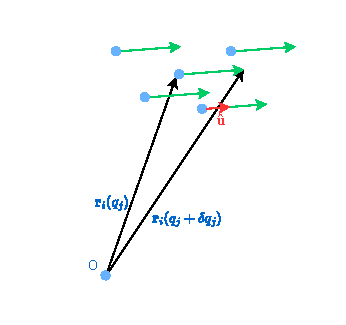
\includegraphics[width=0.4\linewidth]{res/svg/collectivecoord.drawio}
    \caption{Collective coordinate}
\end{figure}
If this is the case all the particles are moving parallel to a single unit vector $\hat{u}$:
\begin{equation}
    \hat{u} = \pdv{ \vec{r}_i}{ q_j}
\end{equation}
\begin{equation}
    \delta \vec{r}_i = \delta q_j \hat{u}
\end{equation}
Also $q_j$ cannot appear in the expression of $T$, hence:
\begin{equation}
    \pdv{T}{q_j}=0
\end{equation}
Changing $q_j$ is a translation that leaves everything untouched (like moving the origin of the axis). Now consider $V=V(q_{\alpha},\cancel{\dot{q}_{\alpha}},t)$:
\begin{equation}
    -\pdv{V}{q_{\alpha}} = Q_{\alpha}
\end{equation}
Let's consider \eleref\;for $q_j$:
\begin{equation}
    \dv{}{t}\underbrace{\pdv{\lagr}{\dot{q}_j}}_{p_j} - \underbrace{\pdv{\lagr}{q_j}}_{-\frac{ \partial V}{\partial q_j}} = 0
\end{equation}
\begin{equation} \label{e:ele_for_qj}
    \dv{}{t}p_j = -\pdv{V}{q_j} = Q_j
\end{equation}
Remembering the definition of $Q_j$:
\begin{equation}
    Q_j = \bigsum_i \vec{F}_i \cdot \underbrace{\pdv{\vec{r}_i}{q_j}}_{\hat{u}} = \vec{F}\cdot \hat{u}
\end{equation}
Similarly from the definition of $p_j$:
\begin{equation}
    p_j = \pdv{\lagr}{\dot{q}_j} = \pdv{}{\dot{q}_j}\brackets{\dfrac{1}{2}\bigsum_i m_i \vec{r}_i^{\;2}} = \dfrac{1}{2}\bigsum_i m_i \pdv{}{\dot{q}_j}(\vec{r}_i^2) = \bigsum_i m_i \vec{r}_i \cdot \underbrace{\pdv{\vec{r}_i}{\dot{q}_j}}_{\hat{u}}
\end{equation}
\begin{equation}
    p_j = \vec{P}\cdot\hat{u}
\end{equation}
Going back to \eqref{e:ele_for_qj}:
\begin{equation}
    \dv{}{t} \brackets{\vec{P} \cdot \hat{u}} = \vec{F}\cdot \hat{u}
\end{equation}
If $q_j$ is also a cyclic coordinate we have:
\begin{equation}
    \pdv{\lagr}{q_j} = 0 \Rightarrow \pdv{[\cancel{T}-V]}{q_j} = \pdv{V}{q_j} = 0
\end{equation}
From this immediately follows:
\begin{equation}
    Q_j = 0 \Rightarrow \dv{p_j}{t} = \dv{}{t} \brackets{\vec{P}\cdot\hat{u}} = 0
\end{equation}
So if $q_j$ is a cyclic and collective coordinate the generalized momentum conjugate to $q_j$ si conserved.
\section{Conservation of the total angular momentum}
Let's consider a specific coordinate $q_j$ such that $\delta q_j$ is a rigid rotation of the system as a whole, about a certain axis as shown:
\begin{figure}[H]
    \centering
    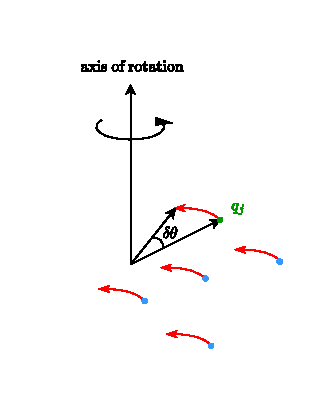
\includegraphics[width=0.4\textwidth]{res/svg/collective_rotation.drawio}
\end{figure}
We can see that $\delta \vec{r}_i$ is a tangential displacement. If we use the angle $\theta$ as our coordinate we can write:
\begin{equation}
    \dv{\vec{r}_i}{t} = \dv{\theta}{t} \hat{u} \cross \vec{r}_i = \dot{q}_j \hat{u} \cross \vec{r}_i
\end{equation}
From which follows:
\begin{equation}
    \delta \vec{r}_i = \delta q_j \hat{u} \cross \vec{r}_i \Rightarrow \pdv{\vec{r}_i}{q_j} = \hat{u} \cross \vec{r}_i
\end{equation}
Also $q_j$ cannot appear in the expression of $T$, hence:
\begin{equation}
    \pdv{T}{q_j} = 0
\end{equation}
Now we consider a system such that $V = V(q_{\alpha},\cancel{\dot{q}_{\alpha}},t)$ and write \eleref\;for $q_j$:
\begin{equation} \label{e:ele_for_angular_momentum}
    \begin{split}
        \dv{}{t}\pdv{\lagr}{\dot{q}_j} - \pdv{\lagr}{q_j} = 0\\[8pt]
        \dv{}{t}\underbrace{\pdv{T}{\dot{q}_j}}_{p_j} - \bbrackets{\underbrace{- \pdv{V}{q_j}}_{Q_j}} = 0
    \end{split}
\end{equation}
Let's explicitly write $Q_j$:
\begin{equation}
    Q_j = \bigsum_i \vec{F}_i \cdot \pdv{\vec{r}_i}{q_j} = \bigsum_i \vec{F}_i \cdot \hat{u} \cross \vec{r}_i
\end{equation}
Inside the summation we have a triple product, hence we can exploit the fact that $\hat{u}$ does not depend on $i$ and also the invariance of the triple product with respect to circular shifts:
\begin{equation}
    \vec{a} \cdot \vec{b} \cross \vec{c} = \vec{c} \cdot \vec{a} \cross \vec{b} = \vec{b} \cdot \vec{c} \cross \vec{a}
\end{equation}
And so we get:
\begin{equation}
    Q_j = \hat{u} \cdot \underbrace{\bigsum_i \vec{r}_i \cross \vec{F}_i}_{\vec{\tau}} = \hat{u} \cdot \vec{\tau}
\end{equation}
Now let's analyse the partial derivative of the kinetic energy:
\begin{equation}
    \pdv{T}{\dot{q}_j} = \pdv{}{\dot{q}_j}\brackets{\dfrac{1}{2}\bigsum_i m_i \vec{r}_i^{\;2}} = \bigsum_i m_i \vec{r}_i \cdot \pdv{\vec{r}_i}{\dot{q}_j} = \bigsum_i m_i \vec{r}_i \cdot \hat{u} \cross \vec{r}_i
\end{equation}
Again we exploit the properties of the triple product and get:
\begin{equation}
    \pdv{T}{\dot{q}_j} =   \hat{u} \cdot \underbrace{\bigsum_i \vec{r}_i \cross m_i \vec{r}_i}_{\vec{L}_0} = \hat{u} \cdot \vec{L}_0
\end{equation}
Finally we can substitute back into \eqref{e:ele_for_angular_momentum}:
\begin{equation}
    \dv{}{t}\brackets{\vec{L}_0 \cdot \hat{u}} = \vec{\tau} \cdot \hat{u}
\end{equation}
This means that if the total torque about a generic axis is zero, then the total angular momentum about that axis is conserved. For example if we let $\hat{u} = \hat{z}$:
\begin{equation}
    \tau_z = 0 \Rightarrow L_z\;\text{is conserved}
\end{equation}
We then notice that if $q_j$ is a cyclic coordinate we have:
\begin{equation}
    Q_j = -\pdv{V}{q_j} = 0 \Rightarrow \vec{\tau} \cdot \hat{u} = 0 \Rightarrow \vec{L}_0 \cdot \hat{u}\;\text{is conserved}
\end{equation}
\section{Noether's theorem}
In the last two sections we arrived to these conclusions:
\begin{itemize}
    \item The conservation of the total momentum is due to an invariance of $\lagr$ to translations
    \item The conservation of the momentum along an axis is due to an invariance of $\lagr$ to translation along that axis
    \item The conservation of the total angular momentum is due to an invariance of $\lagr$ to rotations
    \item The conservation of the angular momentum along an axis is due to an invariance of $\lagr$ to rotations along that axis
    \item If $\lagr$ is invariant with respect to time the energy function is conserved
\end{itemize}
We can easily see the "pattern" arising from those conclusions. Those are all examples of a famous theorem which states:
\begin{theorem}{Noether's theorem}
    For every invariance of $\lagr$ there is a conserved quantity
\end{theorem}
